
\chapter{倾向得分在观测性因果效应研究中的核心作用}\label{chapter::pscore-key}
\chaptermark{倾向得分} 
 
 
\citet{rosenbaum1983central}提出了{\it 倾向得分}这一关键概念，并讨论其在观察性研究因果推断中的作用。该文是统计学引用最多的论文之一，\citet{titterington2013biometrika}将其列为{\it《Biometrika》}过去百年发表论文中被引次数第二高的论文。近年来，其引用量增长很快。 


在独立同分布采样假设下，每个研究单位对应四个随机变量：$\{  X, Z, Y(1), Y(0) \} $。根据概率论基本规则，联合分布可分解为：
\begin{eqnarray*}
&&\pr \{  X, Z, Y(1), Y(0) \}  \\
 &=& \pr(X)  
\times   \pr\{ Y(1), Y(0) \mid X \}   
 \times  \pr\{  Z\mid X, Y(1), Y(0)  \} ,
\end{eqnarray*}
其中：
\begin{enumerate}
\item
 $\pr(X)$为协变量分布； 
 \item
 $\pr\{ Y(1), Y(0) \mid X \}$为在给定协变量$X$时的结果变量分布；
 \item
 $\pr\{  Z\mid X, Y(1), Y(0)  \}$为在给定协变量$X$时的处理分配概率，即处理机制。 
\end{enumerate}
通常我们无需对协变量建模，因为它们属于处理与结果发生前的背景信息。若需进一步分析，则需关注处理机制，这便引出了倾向得分的定义。

\begin{definition}
[倾向得分]\label{def::pscore}
定义
$$
e(X, Y(1), Y(0)   ) = \pr\{  Z=1\mid X, Y(1), Y(0)  \}
$$
为{\it 倾向得分}。在强可忽略性条件下，有
$$
 e(X, Y(1), Y(0)   )  = \pr\{  Z=1\mid X, Y(1), Y(0)  \} = \pr(Z=1 \mid X),
$$
此时倾向得分可简化为
$$
e(X) = \pr(Z=1 \mid X),
$$
即在给定协变量时接受处理的条件概率。  
\end{definition} 

 
\citet{rosenbaum1983central}将$e(X) = \pr(Z=1 \mid X)$作为倾向得分的定义，因其研究重点为强可忽略条件下的观测性研究。即便在强可忽略性不成立时，将$e(X, Y(1), Y(0)   ) = \pr\{  Z=1\mid X, Y(1), Y(0)  \}$视作倾向得分的广义定义亦不失合理性。更多细节可参见问题\ref{hw::principal-unobserved-cov}。 

遵循\citet{rosenbaum1983central}的思路，本章将论证：在可忽略性条件成立时，$e(X)$正是观测性研究中实现因果推断的关键量。

 


\section{倾向得分作为降维工具}

\subsection{理论推导}

\begin{theorem}
\label{thm::pscore-dimreduction}
若$Z\ind \{ Y(1), Y(0)  \} \mid X$，则
$
Z\ind \{ Y(1), Y(0)  \} \mid e(X).
$
\end{theorem}

定理\ref{thm::pscore-dimreduction}指出：若给定协变量$X$后强可忽略性成立，给定标量倾向得分$e(X)$后也成立。可忽略性原本需要同时控制单位的许多背景特征$X$，但定理\ref{thm::pscore-dimreduction}表明，只给定$e(X)$就能消除由$X.$引起的全部混杂。原协变量$X$可以很一般、维数很高，而$e(X)$只是介于$0$与$1$之间的一维标量。倾向得分因此既降低协变量维数，又保留可忽略性。用统计术语说，它是一种{\it 降维}工具。下面先证明定理\ref{thm::pscore-dimreduction}，再介绍降维性质的应用。 





\begin{myproof}{定理}{\ref{thm::pscore-dimreduction}}根据条件独立的定义，只需证明
\begin{eqnarray}
\pr\{ Z=1\mid Y(1), Y(0), e(X)  \} = \pr\{ Z=1\mid e(X)  \} .
\label{eq::pscore-dimreduction}
\end{eqnarray}
\eqref{eq::pscore-dimreduction}左边等于
\begin{eqnarray*}
&&\pr\{ Z=1\mid Y(1), Y(0), e(X)  \}  \\
&=& E\{ Z \mid Y(1), Y(0), e(X)  \}  \\
&=& E\Big[   E\{ Z \mid Y(1), Y(0), e(X) , X  \}  \mid   Y(1), Y(0), e(X)    \Big]  \\
&&\quad  \quad  \quad  \quad   \quad \quad \text{(tower property; see Section \ref{appendix::tower-property})} \\
&=& E\Big[   E\{ Z \mid Y(1), Y(0),   X  \}  \mid   Y(1), Y(0), e(X)    \Big]  \\
&=& E\Big\{    E(Z \mid  X  )  \mid   Y(1), Y(0), e(X)    \Big\}  \quad \text{(strong ignorability)} \\
&=& E\Big\{   e(X) \mid   Y(1), Y(0), e(X)    \Big\} \\
&=& e(X).
\end{eqnarray*}
\eqref{eq::pscore-dimreduction}右边等于
\begin{eqnarray*}
&& \pr\{ Z=1\mid e(X)  \} \\
  &=&  E\{ Z \mid e(X)  \} \\
 &=& E\Big[   E\{ Z \mid e(X), X  \}  \mid e(X)  \Big ] \quad \text{(tower property)} \\
 &=& E\Big\{    E( Z \mid  X )  \mid e(X)  \Big \}   \\
 &=& E\Big\{   e(X)  \mid e(X)  \Big \} \\
 &=& e(X). 
\end{eqnarray*}
因此，\eqref{eq::pscore-dimreduction}的左边等于\eqref{eq::pscore-dimreduction}的右边。 
\end{myproof}


\subsection{倾向得分分层法}
\label{sec::pscore-stratification}




由定理\ref{thm::pscore-dimreduction}可得到简单的倾向得分分层法。先假定倾向得分已知，只取$K$个可能值$\{ e_1,\ldots, e_K \}$，且$K$远小于样本量$n$。此时定理\ref{thm::pscore-dimreduction}化为
$$
Z\ind \{ Y(1), Y(0)  \} \mid e(X) = e_k  \quad (k=1,\ldots, K).
$$
因此，可视为一个分层随机实验：倾向得分各层内有$K$个独立的完全随机实验。可按以$e(X)$分层的实验方法分析观察性数据。 


一般而言，倾向得分未知且不离散，通常拟合$\pr(Z = 1\mid X)$的统计模型，例如二元$Z$对$X$的逻辑回归，得到估计$\hat{e}(X)$。它可能有与样本量一样多的不同取值，但可离散化以近似前面的简单情形。例如，按$K$个分位数区间离散化，得到$\hat{e}'(X)$：若$ \hat{e}(X_i)$介于各$\hat{e}(X_i)$的$(k-1)/K$与$k/K$分位数之间，就令
$
\hat{e}'(X_i) = e_k,
$
其中相应的层代表值为$\hat{e}(X)$的$k/K$分位数。此时近似有
$$
Z\ind \{ Y(1), Y(0)  \} \mid \hat{e}'(X) = e_k  \quad (k=1,\ldots, K).
$$
可按以$\hat{e}'(X)$分层的随机实验分析。由于给定$\hat{e}'(X)$后的可忽略性只近似成立，还可用协变量作回归调整，消除偏差并提高效率。具体可在每层计算\citet{lin2013}的估计量，再加权平均得到最终估计，见第\ref{sec::covariate-SRE}节。 


 




倾向得分未知时，必须拟合统计模型获得$\hat{e}(X)$，最终估计因而依赖模型设定。不过，倾向得分分层主要依赖估计得分的正确排序，而非精确数值，因此相对其他方法较稳健。许多数值例子呈现了这一性质，但文献中仍缺乏对其严格的量化。 




实践中如何选择$K$？$K$过小，给定$\hat{e}'(X)$后，可忽略性甚至未必近似成立；$K$过大，每层单位不足，许多层可能只有处理或只有对照，因此存在权衡。沿用\citet{cochran1968effectiveness}的直观论证，\citet{rosenbaum1983central}和\citet{rosenbaum1984reducing}建议$K=5$，在许多情形下能消除大量偏差。但数据极大时，固定$K$会使分层估计仍有偏\citep{lunceford2004stratification}，所以只要各层保有足够处理与对照单位，就可以增大$K$。\citet{wang2020robust}提出贪心选择$K$：取使分层估计量仍有定义的最大层数，但这一过程的严格理论尚未完全建立。 




另一个实际问题是如何计算倾向得分分层估计的标准误。有研究者以离散得分$\hat{e}'(X)$为条件，按分层随机实验计算标准误，实际上忽略了倾向得分估计的不确定性。这往往高估真实方差，因为文献中有一个出乎意料的结论：使用估计倾向得分反而可降低平均因果效应估计的渐近方差\citep{su2023estimated}。也有研究者对整个过程作自助法，以计入全部不确定性；但由于估计量具有离散性，这一自助法的理论仍不清楚。 
 
 
 
 \subsection{应用实例}\label{sec::application-pscore-stratification}


为演示该方法的实践效果，现以\ref{eg::chan-bmi-ATE}为例重现分析： 
\begin{lstlisting}
> nhanes_bmi = read.csv("nhanes_bmi.csv")[, -1]
> z = nhanes_bmi$School_meal
> y = nhanes_bmi$BMI
> x = as.matrix(nhanes_bmi[, -c(1, 2)])
> x = scale(x)
\end{lstlisting}
例\ref{eg::chan-bmi-ATE}介绍了数据集的协变量。处理\ri{School_meal}表示是否参加学校供餐计划，结果\ri{BMI}为 BMI。 



\begin{figure}
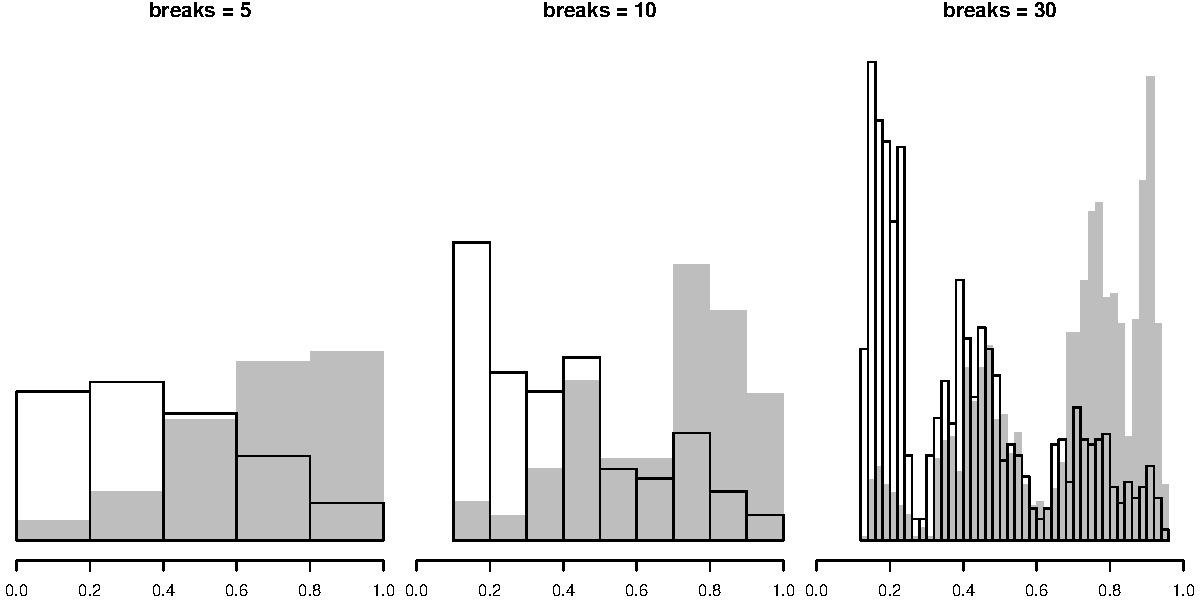
\includegraphics[width = \textwidth]{figures/pscore_stratified_hist.pdf}
\caption{基于\ri{nhanes_bmi}数据的倾向得分分布直方图：白色为对照组、灰色为处理组}\label{fig::pscore_bmi}
\end{figure}


图\ref{fig::pscore_bmi}画出了采用不同组数$(K=5,10,30)$的估计倾向得分直方图。利用第\ref{chapter::stratification-poststratification}章分析分层随机实验的\ri{Neyman_SRE}函数，可以对$K \in \{5, 10, 20, 50, 80 \}$的不同选择计算分层点估计与标准误：
\begin{lstlisting}
> pscore = glm(z ~ x, family = binomial)$fitted.values
> n.strata = c(5, 10, 20, 50, 80)
> strat.res = sapply(n.strata, FUN = function(nn){
+   q.pscore = quantile(pscore, (1:(nn-1))/nn)
+   ps.strata = cut(pscore, breaks = c(0,q.pscore,1), 
+                   labels = 1:nn)
+   Neyman_SRE(z, y, ps.strata)})
> 
> rownames(strat.res) = c("est", "se")
> colnames(strat.res) = n.strata
> round(strat.res, 3)
         5     10     20     50     80
est -0.116 -0.178 -0.200 -0.265 -0.204
se   0.283  0.282  0.279  0.272     NA
\end{lstlisting}
将$K$从$5$增至$50$降低了标准误。但不能极端地取$K=80$，因为某些层只有一个处理或对照单位，标准误无法定义。上述估计表明供餐计划对 BMI 的效应为负，但不显著。 


亦可将此法与三种传统回归法对比：不校正协变量的基础估计、Fisher法、Lin法。 
\begin{lstlisting}
> DiM = lm(y ~ z)
> Fisher = lm(y ~ z + x)
> Lin = lm(y ~ z + x + z*x)
> res.regression = c(coef(DiM)[2], hccm(DiM)[2, 2]^0.5,
+                    coef(Fisher)[2], hccm(Fisher)[2, 2]^0.5,
+                    coef(Lin)[2], hccm(Lin)[2, 2]^0.5)
> res.regression = matrix(res.regression,
+                         nrow = 2, ncol = 3)
> rownames(res.regression) = c("est", "se")
> colnames(res.regression) = c("naive", "fisher", "lin")
> round(res.regression, 3)   
    naive fisher    lin
est 0.534  0.061 -0.017
se  0.225  0.227  0.226
\end{lstlisting} 
由于协变量严重不平衡，朴素均值差与其他方法差异很大。Fisher 估计的点估计仍为正，但不显著；Lin 估计与倾向得分分层估计给出相同的定性结论。分层估计对不同$K$的选择较稳定。 




\section{倾向得分加权法}

\subsection{理论推导}

\begin{theorem}
\label{thm::pscore-weighting}
若满足$Z\ind \{ Y(1), Y(0)  \} \mid X$且$0<e(X)<1$，则
$$
E\{  Y(1) \} =  E\left\{  \frac{ZY}{e(X)}  \right\},\quad
E\{  Y(0) \} =  E\left\{  \frac{(1-Z)Y}{1-e(X)}  \right\} ,
$$
进而可得
$$
\tau = E\{  Y(1) -  Y(0) \} =  E\left\{  \frac{ZY}{e(X)} - \frac{(1-Z)Y}{1-e(X)}   \right\} .
$$
\end{theorem}


证明定理\ref{thm::pscore-weighting}前，须注意额外假设$0<e(X)<1$，称为{\it 重叠性}或{\it 正值性}条件。若某些$X$使$e(X)=0$或$1$成立，定理\ref{thm::pscore-weighting}会出现零分母。这并非倾向得分加权识别公式特有的要求：尽管定理\ref{thm::identification-formula}未明说，\eqref{eq::nonparametric-identification-tau}中识别$\tau$所需的条件期望$E(Y\mid Z=1, X)$与$ E(Y\mid Z=0, X)$，也只有在$0< e(X) < 1$时都有良好定义。重叠性可视为保证定理\ref{thm::identification-formula}和\ref{thm::pscore-weighting}公式有定义的技术条件，也涉及观察性因果推断的哲学问题。若单位$i$满足$e(X_i)=1$，总能观测其处理潜在结果$Y_i(1)$，却永远不能观测其对照潜在结果$Y_i(0)$。甚至$Y_i(0)$本身也可能没有明确含义，使单位$i$的因果效应定义变得模糊。\citet{king2006dangers}将$e(X_i)=1$时的$Y_i(0)$称为{\it 极端反事实}，并讨论了它对因果推断的危害。单位$i$满足$e(X_i)=0$时也有类似问题。 
 
 
$Z\ind \{ Y(1), Y(0)  \} \mid X$要求观测到足够协变量，以保证处理与潜在结果条件独立；$0<e(X)<1$则要求给定协变量后，处理仍保有随机性。事实上，\citet{rosenbaum1983central}对强可忽略性的原始定义同时包含这两个条件，现代文献往往将它们分开陈述。 
 


 

\begin{myproof}{定理}{\ref{thm::pscore-weighting}}这里只证明$E\{ Y(1) \}$的结论，$E\{ Y(0) \}$的证明类似。有
\begin{eqnarray*}
&&E\left\{  \frac{ZY}{e(X)}  \right\} \\
&=& E\left\{  \frac{ZY(1)}{e(X)}  \right\} \\
&=& E\left[ E\left\{  \frac{ZY(1)}{e(X)}  \mid X \right\}  \right]  \quad \text{(tower property)} \\
&=& E\left[  \frac{1}{e(X)}   E\left\{   ZY(1)  \mid X \right\}  \right]   \\
&=& E\left[  \frac{1}{e(X)}   E( Z  \mid X ) E\left\{   Y(1)  \mid X \right\}  \right]  \quad \text{(strong ignorability)} \\\\
&=& E\left[  \frac{1}{e(X)}   e(X) E\left\{   Y(1)  \mid X \right\}  \right] \\
&=& E\left[ E\left\{   Y(1)  \mid X \right\}  \right] \\
&=& E\{   Y(1) \}. 
\end{eqnarray*}
\end{myproof}



\subsection{逆倾向得分加权估计法}\label{sec::ipw-estimators}

由定理\ref{thm::pscore-weighting}，得到平均因果效应的矩估计量
$$
\hat{\tau}^\textup{ht} = \frac{1}{n} \sumn \frac{Z_i Y_i}{ \hat{e}(X_i) }
- \frac{1}{n} \sumn \frac{ (1-Z_i) Y_i}{ 1 - \hat{e}(X_i) } ,
$$
其中$\hat{e}(X_i)$为倾向得分估计。这称为逆倾向得分加权（IPW）估计量，也称 Horvitz--Thompson（HT）估计量。\citet{horvitz1952generalization}在抽样调查中提出它，\citet{rosenbaum1987model}将其用于观察性研究的因果推断。 


但$\hat{\tau}^\textup{ht}$有不少问题，特别是不具有对结果平移变换的不变性。命题\ref{prop::no-invariance-HT}精确表述了这一问题，证明留作习题\ref{hw::hajek-weights}。 

\begin{proposition}
[HT估计法的非不变性]
\label{prop::no-invariance-HT}
将$Y_i$改为$Y_i+c$，其中$c$为常数，则 HT 估计量$\hat{\tau}^\textup{ht}$变为$\hat{\tau}^\textup{ht} + c (\hat{ 1 }_\textsc{T} - \hat{ 1 }_\textsc{C})$，其中
$$
\hat{ 1 }_\textsc{T}=   \frac{1}{n} \sumn \frac{Z_i }{ \hat{e}(X_i) } ,\quad
\hat{ 1 }_\textsc{C} =\frac{1}{n} \sumn \frac{ (1-Z_i) }{ 1 - \hat{e}(X_i) }   
$$
可看作常数$1$的两个不同估计。 
\end{proposition}

命题\ref{prop::no-invariance-HT}采用了有些特别的记号$\hat{ 1 }_\textsc{T} $与$ \hat{ 1 }_\textsc{C}$：使用真实倾向得分时，这两项的期望都为 1，见习题\ref{hw::hajek-weights}。但有限样本下，$\hat{ 1 }_\textsc{T} - \hat{ 1 }_\textsc{C}$一般不为零。给所有结果加同一个常数本不应改变平均因果效应，HT 估计却依赖$c.$，因此不够理想。简单修正是分别用$\hat{ 1 }_\textsc{T}  $和$\hat{ 1 }_\textsc{C} $归一化权重，得到
$$
\hat{\tau}^\textup{hajek} = \frac{  \sumn \frac{Z_i Y_i}{ \hat{e}(X_i) }  }{  \sumn \frac{Z_i }{ \hat{e}(X_i) } }
- \frac{  \sumn \frac{ (1-Z_i) Y_i}{ 1 - \hat{e}(X_i) }  }{  \sumn \frac{ 1-Z_i}{ 1 - \hat{e}(X_i) }  }.
$$
这就是\citet{hajek1971comment}在不等概率抽样背景下提出的 Hájek 估计量。可以验证，它对平移变换不变：把$Y_i$换成$Y_i + c$后，$\hat{\tau}^\textup{hajek}$不变，见习题\ref{hw::hajek-weights}。许多数值研究还发现，在有限样本中$\hat{\tau}^\textup{hajek}$比$\hat{\tau}^\textup{ht}$稳定得多。 





\subsection{IPW方法的缺陷与因果推断的根本难题}
\label{sec::ipw-problem}


许多渐近分析要求{\it 强重叠性}条件
$$
0<  \alpha_\textsc{L} \leq e(X) \leq  \alpha_\textsc{U} < 1,
$$
即真实倾向得分与$0$和$1$保持正距离。但\citet{d2017overlap}指出，尤其在协变量较多时，这是相当强的假设，第\ref{chapter::overlap}章将详述。 


即使真实倾向得分满足强重叠性，估计倾向得分仍可能接近$0$或$1$，使加权估计量趋于极端，有限样本表现很不稳定。一种做法是截断得分，改为
$$
 \max\Big[  \alpha_\textsc{L},   \min\{   \hat{e}(X_i), \alpha_\textsc{U} \}   \Big] ,
$$
另一种做法是修剪样本，删除$\hat{e}(X_i)$位于区间$[\alpha_\textsc{L},   \alpha_\textsc{U}  ]$之外的单位。\citet{crump2009dealing}建议$  \alpha_\textsc{L} = 0.1$与$\alpha_\textsc{U} = 0.9 $，\citet{kurth2005results}建议$  \alpha_\textsc{L} = 0.05$与$\alpha_\textsc{U} = 0.95 $，\citet{yang2018asymptotic}建立了一些修剪的渐近理论。总的来说，修剪虽然常使 IPW 更稳定，也给分析增加了任意性。 




 \subsection{应用实例}\label{sec::application-pscore-weighting}


以下代码实现IPW估计及其自助法标准误计算： 
\begin{lstlisting}
ipw.est = function(z, y, x, truncps = c(0, 1))
{
  ## fitted propensity score
  pscore   = glm(z ~ x, family = binomial)$fitted.values
  pscore   = pmax(truncps[1], pmin(truncps[2], pscore))
  
  ace.ipw0 = mean(z*y/pscore - (1 - z)*y/(1 - pscore))
  ace.ipw  = mean(z*y/pscore)/mean(z/pscore) - 
    mean((1 - z)*y/(1 - pscore))/mean((1 - z)/(1 - pscore))
  
  return(c(ace.ipw0, ace.ipw))     
}


ipw.boot = function(z, y, x, n.boot = 500, truncps = c(0, 1))
{
  point.est  = ipw.est(z, y, x, truncps)
  
  ## nonparametric bootstrap
  n.sample   = length(z)
  x          = as.matrix(x)
  boot.est   = replicate(n.boot, {
    id.boot = sample(1:n.sample, n.sample, replace = TRUE)
    ipw.est(z[id.boot], y[id.boot], x[id.boot, ], truncps)
  })
  boot.se    = apply(boot.est, 1, sd)
  
  res = cbind(point.est, boot.se)
  colnames(res) = c("est", "se")
  rownames(res) = c("HT", "Hajek")
  
  return(res)
}
\end{lstlisting}

重新考虑例\ref{eg::chan-bmi-ATE}，在不同倾向得分截断下计算 IPW 估计。下面给出截断范围分别为$(0,1)$、$(0.01, 0.99)$、$(0.05, 0.95)$和$(0.1, 0.9)$时的两种加权估计及自助法标准误：
\begin{lstlisting}
> trunc.list = list(trunc0 = c(0,1), 
+                   trunc.01 = c(0.01, 0.99), 
+                   trunc.05 = c(0.05, 0.95), 
+                   trunc.1 = c(0.1, 0.9))
> trunc.est = lapply(trunc.list,
+                    function(t){
+                      est = ipw.boot(z, y, x, truncps = t)
+                      round(est, 3)
+                    })
> trunc.est
$trunc0
         est    se
HT    -1.516 0.496
Hajek -0.156 0.258

$trunc.01
         est    se
HT    -1.516 0.501
Hajek -0.156 0.254

$trunc.05
         est    se
HT    -1.499 0.501
Hajek -0.152 0.255

$trunc.1
         est    se
HT    -0.713 0.425
Hajek -0.054 0.246
\end{lstlisting}
HT 估计与此前所有其他估计差异很大，点估计的绝对值似乎过大。除采用$(0.1, 0.9)$截断外，它们都呈显著负向效应。这说明了 HT 估计的不稳定性。 



\section{倾向得分的平衡特性}


\subsection{理论推导}



\begin{theorem}
\label{thm::pscoreASbscore}
倾向得分满足
$$
Z\ind X \mid e(X) .
$$
此外，对任意函数$h(\cdot)$，只要\eqref{eq::balancehX}两侧所需矩存在，就有
\begin{eqnarray}
E\left\{   \frac{Zh(X)}{e(X)}   \right\} = E\left\{   \frac{(1-Z)h(X)}{1-e(X)}   \right\}
\label{eq::balancehX}
\end{eqnarray} 
\end{theorem}

定理\ref{thm::pscoreASbscore}不要求可忽略性，只涉及处理$Z$和协变量$X$。定理\ref{thm::pscoreASbscore}的第一部分指出，给定倾向得分后，处理指标与协变量独立，故在相同倾向得分水平内，处理组与对照组的协变量分布平衡。定理\ref{thm::pscoreASbscore}的第二部分给出了加权形式的等价平衡关系。下面证明定理\ref{thm::pscoreASbscore}。  


\begin{myproof}{定理}{\ref{thm::pscoreASbscore}}首先证明$Z\ind X \mid e(X)$，即
\begin{eqnarray}
\pr\{Z=1\mid X, e(X)\} = \pr\{Z=1\mid  e(X)\}.
\label{eq::balance1}
\end{eqnarray}
采用与定理\ref{thm::pscore-dimreduction}类似的步骤，\eqref{eq::balance1}左侧为
$$
\pr\{Z=1\mid X, e(X)\} = \pr( Z=1\mid X ) = e(X),
$$
\eqref{eq::balance1}右侧为
\begin{eqnarray*}
\pr\{Z=1\mid  e(X)\} &=& E\{  Z\mid  e(X) \}  \\
&=& E\Big[ E\{  Z\mid X,  e(X) \} \mid e(X) \Big] \\
&=& E\Big[ E\{  Z\mid X  \} \mid e(X) \Big] \\
&=& E\Big[ e(X) \mid e(X) \Big] \\
&=& e(X). 
\end{eqnarray*}
所以\eqref{eq::balance1}成立。 

其次证明\eqref{eq::balancehX}，可仿照定理\ref{thm::pscore-weighting}的证明。但利用定理\ref{thm::pscore-weighting}，还有更简单的论证：将$h(X)$视为结果时，其两个潜在结果完全相同，且可忽略性$Z\ind \{  h(X), h(X) \}  \mid X$成立。\eqref{eq::balancehX}左右之差就是$Z$对$h(X)$的平均因果效应，必为零。 
\end{myproof}





\subsection{协变量均衡性验证}
\label{sec::balance-check-bmi}

定理\ref{thm::pscoreASbscore}虽易证明，定理\ref{thm::pscoreASbscore}对实际分析却有重要启示。在查看结果数据前，就可通过数据中的协变量平衡，检查倾向得分模型是否足够合理。\citet{rubin2007design}将其视为观察性研究的设计阶段，\citet{rubin2008objective}认为，这一阶段不涉及结果值，能使因果推断更客观。\footnote{这是一项实用建议，但如何量化这种客观性并不完全清楚。} 


倾向得分分层中，得到离散估计得分$\hat{e}'(X)$，并近似有
$$
Z\ind X\mid \hat{e}'(X) = e_k\quad (k=1,\ldots, K).
$$
因此，可以检查每一得分层内，处理组与对照组的协变量分布是否相同。 


倾向得分加权中，可把$h(X)$视为伪结果，估计处理对$h(X)$的平均因果效应。由于$h(X)$上的真实平均因果效应为$0$，估计应当与$0$无显著差异。常用的$h(X)$选择是$X$。 




再次考虑例\ref{eg::chan-bmi-ATE}。采用$K=5$作倾向得分分层后，两组所有协变量都较好地平衡；Hájek 估计也有类似结果。唯一例外是图\ref{fig::balance-check}中的第七个协变量\ri{Food_Stamp}。图\ref{fig::balance-check}给出了平衡检查结果。 

\begin{figure}
\centering
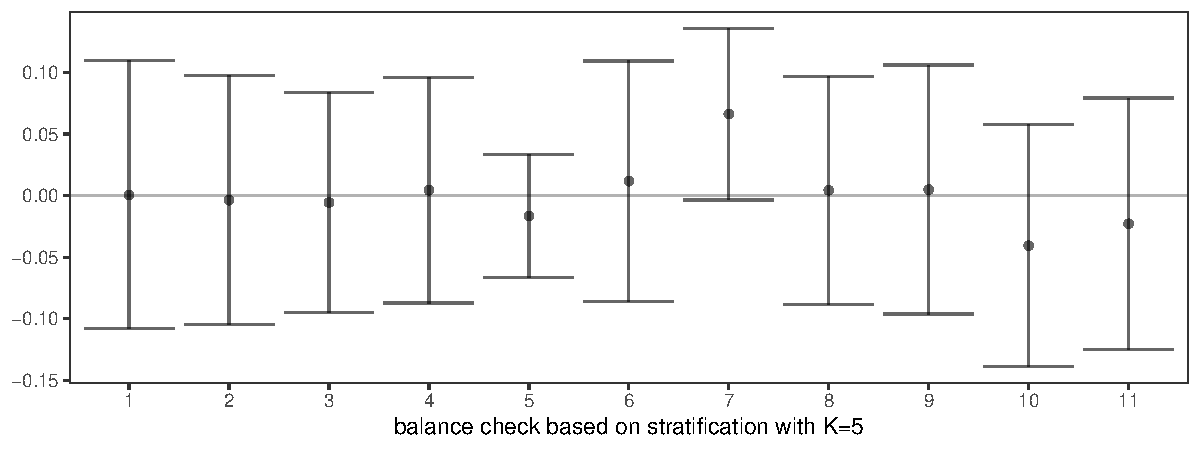
\includegraphics[width = \textwidth]{figures/balance_PSstratification5.pdf}
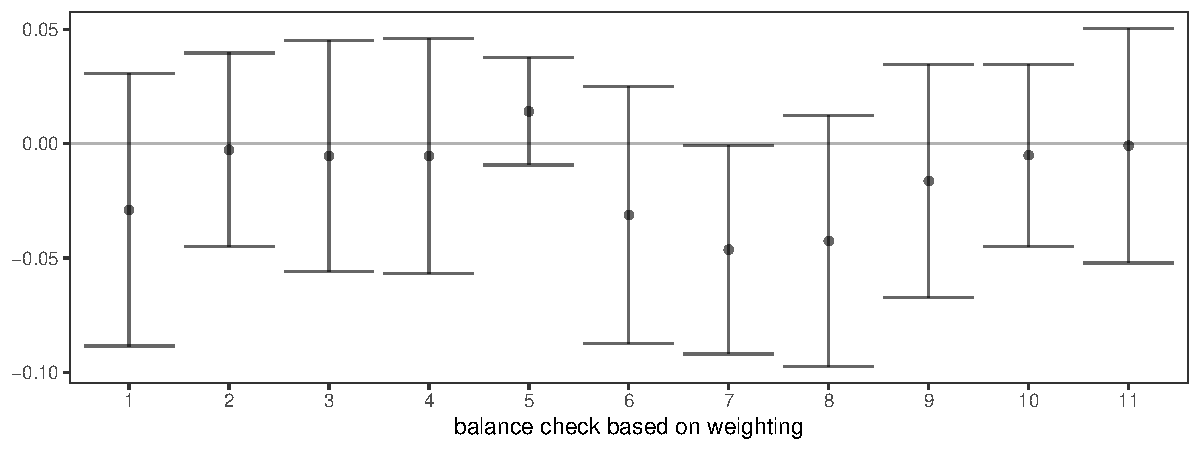
\includegraphics[width = \textwidth]{figures/balance_PShajek.pdf}
\caption{协变量均衡性检验结果：平均因果效应点估计及95\% 协变量上的平均因果效应置信区间}\label{fig::balance-check}
\end{figure}

 

 

 
 
 \section{作业习题}
 
 
 
 
 \paragraph{定理\ref{thm::pscore-dimreduction}的另一版本} \label{hw::principal-unobserved-cov}
 证明
\begin{equation}
\label{eq::principal-covariate-ind}
 Z\ind \{  Y(1), Y(0) , X\}  \mid e(X, Y(1), Y(0)   ) .
\end{equation}  
 
 注：这个结论无需强可忽略性，且蕴含
$$
  Z\ind \{  Y(1), Y(0) \}  \mid  \{ X,   e(X, Y(1), Y(0)  \} .
 $$
\citet{rosenbaum2020modern}与\citet{rosenbaum2023propensity}指出了\eqref{eq::principal-covariate-ind}的结论，将$e(X, Y(1), Y(0)   ) $称为{\it 主要未观测协变量}。 
 
 
 
\paragraph{定理\ref{thm::pscore-dimreduction}的另一版本} 

定理\ref{thm::pscore-dimreduction}在强可忽略性下成立，可忽略性下也有类似结果：若给定协变量$X$后可忽略性成立，则给定标量倾向得分$e(X)$后也成立。 

\begin{theorem}
\label{thm::pscore-dimension-reduction-weak-ig}
若对$z=0,1$有$Z\ind Y(z)  \mid X$，则对$z=0,1$有
$
Z\ind Y(z)\mid e(X)
$ 
\end{theorem} 


证明定理 \ref{thm::pscore-dimension-reduction-weak-ig}。



 
 \paragraph{IPW估计法相关问题}
\label{hw::hajek-weights} 
 
本题涉及第\ref{sec::ipw-estimators}节的 HT 估计。先证明命题\ref{prop::no-invariance-HT}，再证明
\begin{eqnarray*} 
E\left\{ \frac{1}{n} \sumn \frac{Z_i }{e(X_i) } \right\} =1,\quad
E\left\{  \frac{1}{n} \sumn \frac{ (1-Z_i) }{ 1 - e(X_i) }  \right\} = 1.
\end{eqnarray*}
最后证明，给所有观测结果$Y_i$加常数$c$后，Hájek 估计量$
\hat{\tau}^\textup{hajek} 
$保持不变。 


\paragraph{重新分析\citet{Rosenbaum::1983JRSSB}}



表\ref{table::rr1983table1}来自\citet{Rosenbaum::1983JRSSB}，研究冠状动脉搭桥手术相较药物治疗，对心导管检查后六个月功能改善的因果效应。研究者先用 74 个观测协变量估计倾向得分，再按离散得分划为 5 层。处理与结果均为二元变量，因此将数据列成表。根据表\ref{table::rr1983table1}估计平均因果效应，并报告 95\% 置信区间。 



\begin{table}
\caption{\citet{Rosenbaum::1983JRSSB}之表1}\label{table::rr1983table1}
\begin{tabular}{clcc}
\hline 
按$\hat{e}(X)$分层 & 处理方式 &  患者人数 & 改善率\\
\hline 1 & 手术 & 26 & 0.54 \\
& 药物 & 277 & 0.35 \\
2 & 手术 & 68 & 0.70 \\
& 药物 & 235 & 0.40 \\
3 & 手术 & 98 & 0.70 \\
& 药物 & 205 & 0.35 \\
4 & 手术 & 164 & 0.71 \\
& 药物 & 139 & 0.30 \\
5 & 手术 & 234 & 0.70 \\
& 药物 & 69 & 0.39 \\
\hline
\end{tabular}
\end{table}


注：感兴趣的读者可在读完第\ref{part::challenges-os}部分后，通读\citet{Rosenbaum::1983JRSSB}的论文。这是因果推断敏感性分析的经典文献。 

 


\paragraph{均衡得分与倾向得分的理论关联}
\label{hw::balancingscore-rr1983}


\citet{rosenbaum1983central}首创{\it 均衡得分}概念：

\begin{definition}
[均衡得分]\label{def::balancing-score}
  若
$$
  Z\ind X\mid b(X).
  $$
则称$b(X)$为平衡得分。
\end{definition}

定义\ref{def::balancing-score}中，$b(X)$可为标量或向量。显然，$b(X) = X$本身就是平衡得分，但没有简化原协变量，实用价值有限。由定理\ref{thm::pscoreASbscore}，倾向得分是平衡得分的特例。更有意思的是，\citet{rosenbaum1983central}证明倾向得分是最粗的平衡得分，见下面的定理\ref{thm::balancingscore}，其中包含定理\ref{thm::pscoreASbscore}这一特例。 


\begin{theorem}
\label{thm::balancingscore}
$b(X)$是平衡得分，当且仅当$b(X)$至少与$e(X)$同样精细，即存在函数$f(\cdot)$使$e(X) = f(b(X))$。 
\end{theorem}


定理\ref{thm::balancingscore}与亚组分析有关。除平均因果效应$\tau$，也可能关心亚组效应，例如分别估计男孩与女孩的平均因果效应。不失一般性，令$X$的第一分量表示是否为女孩，目标为
$$
\tau(x_1) = E\{ Y(1) - Y(0) \mid X_1 = x_1  \},\quad (x_1=1,0).
$$
由定理\ref{thm::balancingscore}，在可忽略性下还有
\begin{equation}
\label{eq::subgroup-ignorability}
Z\ind \{ Y(1) , Y(0) \} \mid e(X), X_1
\end{equation}
因为$b(X) = \{e(X), X_1\}$比$e(X)$更精细，所以也是平衡得分。\eqref{eq::subgroup-ignorability}的条件独立性保证，在$X_1$的每个水平内，给定倾向得分后可忽略性仍成立。因此，可在$X_1$的各水平内分别作同样的倾向得分分析，得到两个亚组效应的估计。 


根据上述动机，证明定理\ref{thm::balancingscore}。 


\paragraph{亚组效应估计的基础问题}

本题与习题\ref{hw::balancingscore-rr1983}有关，但可独立完成。 

考虑协变量为$X = (X_1, X_2)$的标准观察性研究，其中$X_1$是二元亚组指标，例如是否为统计学专业，$X_2$为其余协变量。目标参数是亚组因果效应
$$
\tau(x_1) = E\{ Y(1) - Y(0) \mid X_1 = x_1  \},\quad (x_1=1,0).
$$
证明
$$
\tau(x_1) =  E\left\{   \frac{  1(X_1 = x_1) ZY}{ e(X) }   - \frac{  1(X_1 = x_1) (1-Z)Y}{ 1 -  e(X) }    \right\} \Big /  \pr(X_1 = x_1)
$$
并给出$\tau(x_1) $对应的 HT 和 Hájek 估计量。 



 \paragraph{推荐阅读}
 
 
本章标题与\citet{rosenbaum1983central}的经典论文相同，多数结论直接取自该文。  


\citet{rubin2007design}与\citet{rubin2008objective}强调，观察性研究的设计阶段对更客观的因果推断很重要。 
 
